\chapter{Long Term Evolution}
\label{chap:lte}

\section{Digital Communication System Overview}
\label{lte:digicomm}

All the information in this chapter was acquired in the \ref{sklar2001} and in the
online lectures of \textit{MIT Opencourseware} \cite{ocw:digicomm}.

The purpose of any Communication System is to transport an information bearing
signal from a source to a user destination via a communication channel. Being
Transmitter, Receiver and Channel the three basic elements of every
communication systems whose block diagram can be seen in figure
\ref{fig:digicomsimple}.\\

%esquema básico do sistema de comunicação
\begin{figure}[htbp]
    \centering
    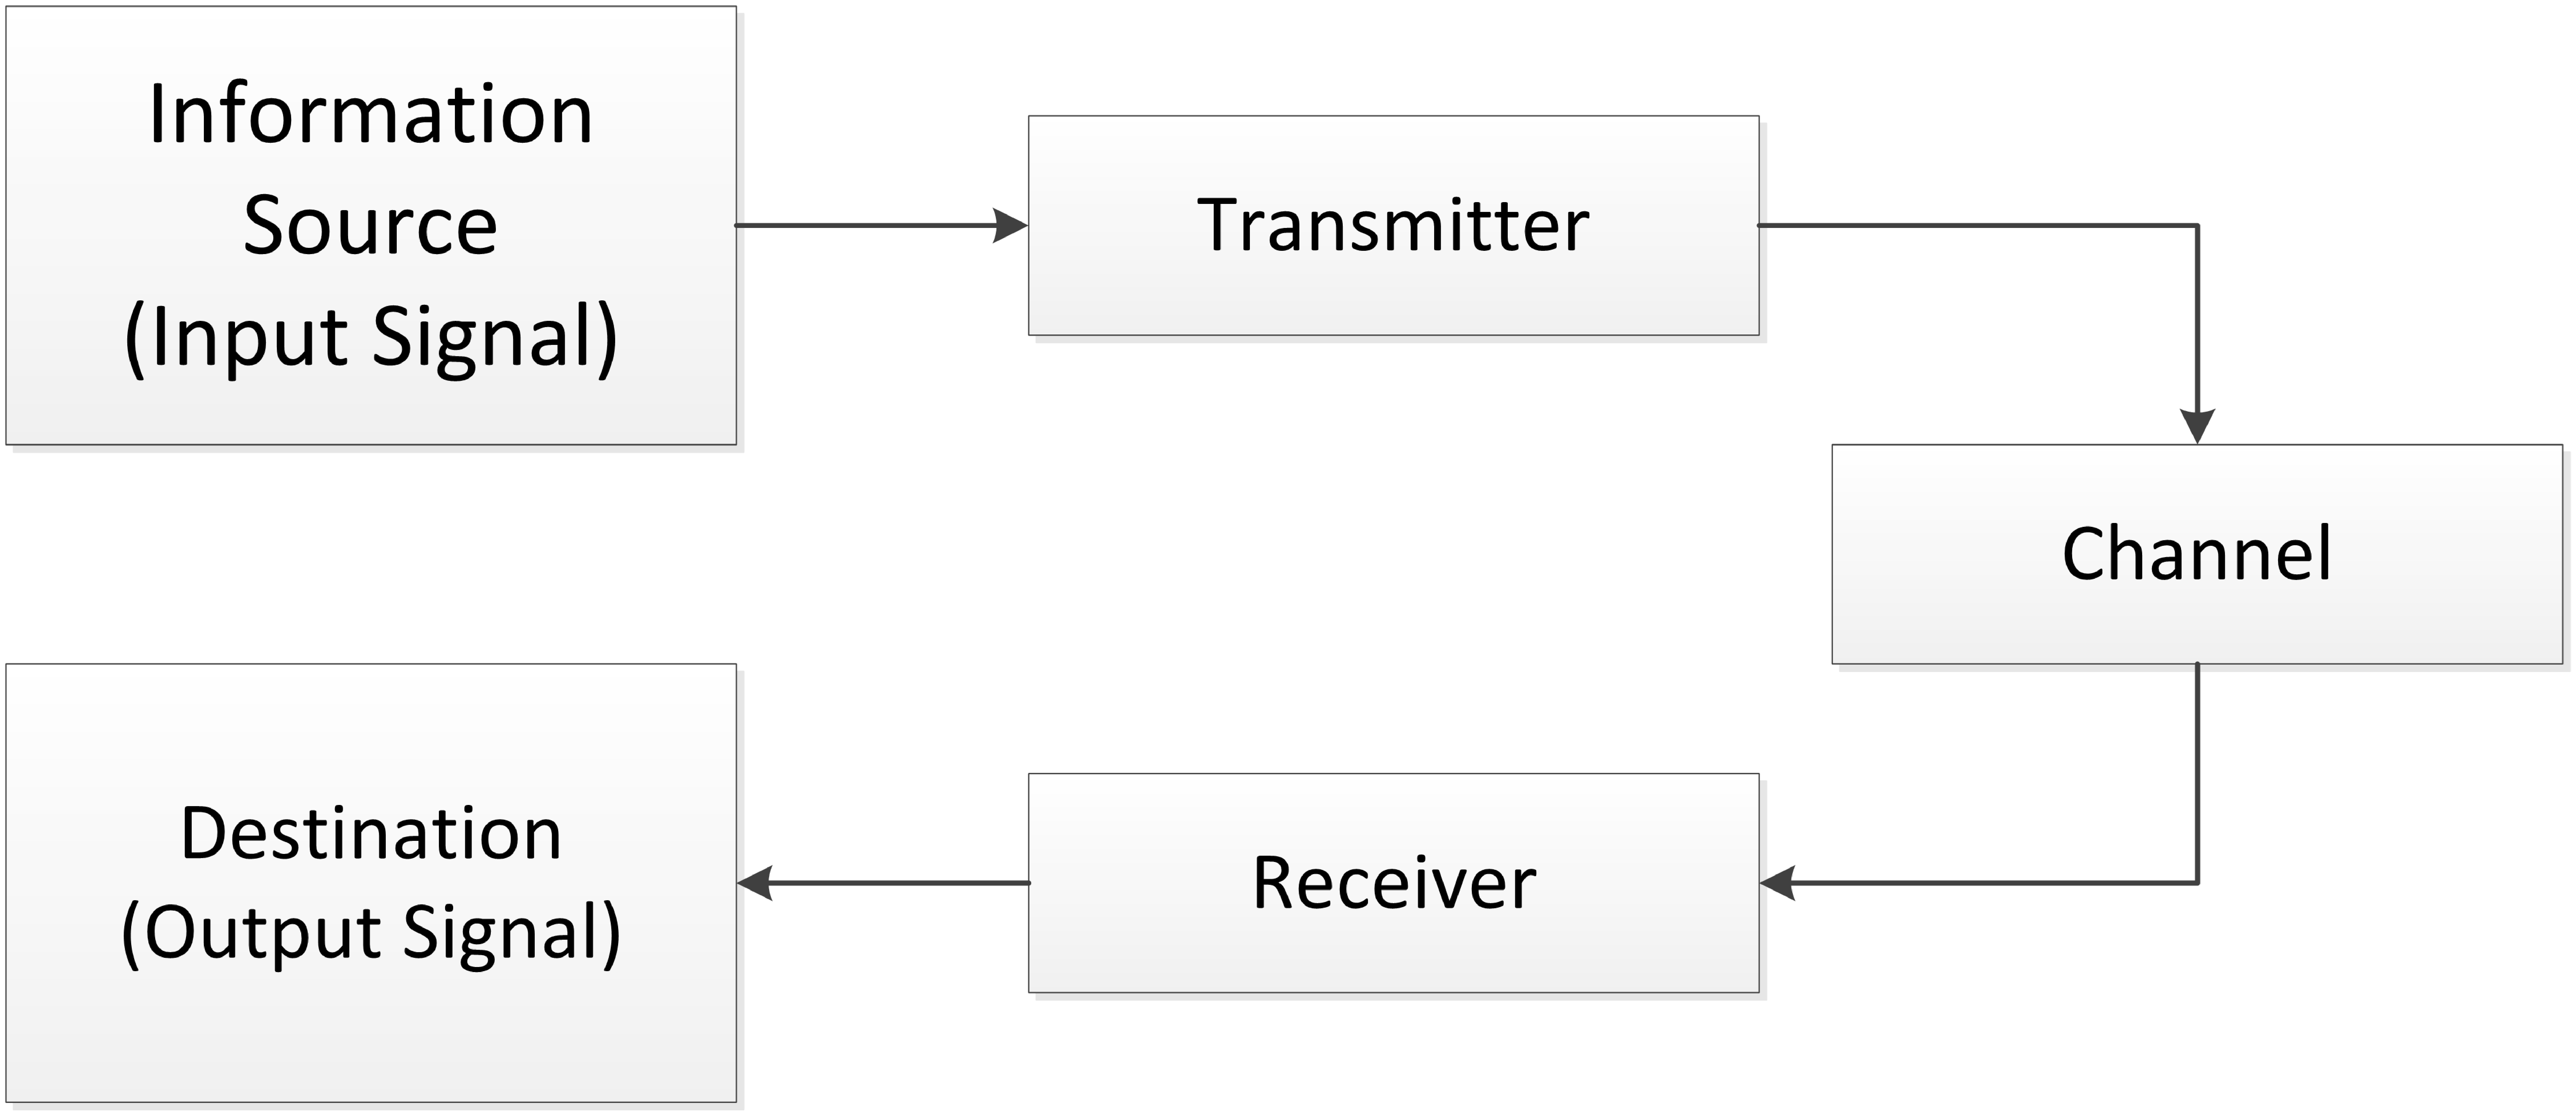
\includegraphics[width=0.65\textwidth]{./figures/digicom_simple}
    \caption{ A simple Digital Communication System Block Diagram
    \label{fig:digcomsimple}}
\end{figure}

The overall purpose of the system is to transfer information from one point (
Source) to another point, the destination.The message produced by a source,
normally, it is a digital message, usually binary, thus not electrical. Hence an
input transducer is used for converting the message to a time-varying electrical
quantity called message signal. Similarly, at the destination point,another
transducer converts the electrical waveform to the appropriate message.\\

The transmitter is located at one point in space, the receiver is located at
some other point separate from the transmitter, and the channel is the medium
that provides the electrical connection between them. Its purpose is to
transform the message signal produced by the source of information into a form
suitable for transmission over the channel.\\

The received signal is normally corrupted version of the transmitted signal,
which is due to channel imperfections, noise and interference from other
sources.It has the task of operating on the received signal so as to reconstruct
a recognizable form of the original message signal and to deliver it to the user
destination.\\

Communication Systems are divided into 3 categories:

\begin{enumerate}

  \item Analog Communication Systems are designed to transmit analog information
  using analog modulation methods, FM and AM, common radio.

  \item Digital Communication Systems are designed for transmitting digital
  information using digital modulation schemes, like FSK and PSK.

  \item Hybrid Systems that use digital modulation schemes for transmitting
  sampled and quantized values of an analog message signal.

\end{enumerate}

\subsection{Elements of Digital Communications Systems}

%block diagram of a digital communication system
\begin{figure}[htbp]
    \centering
    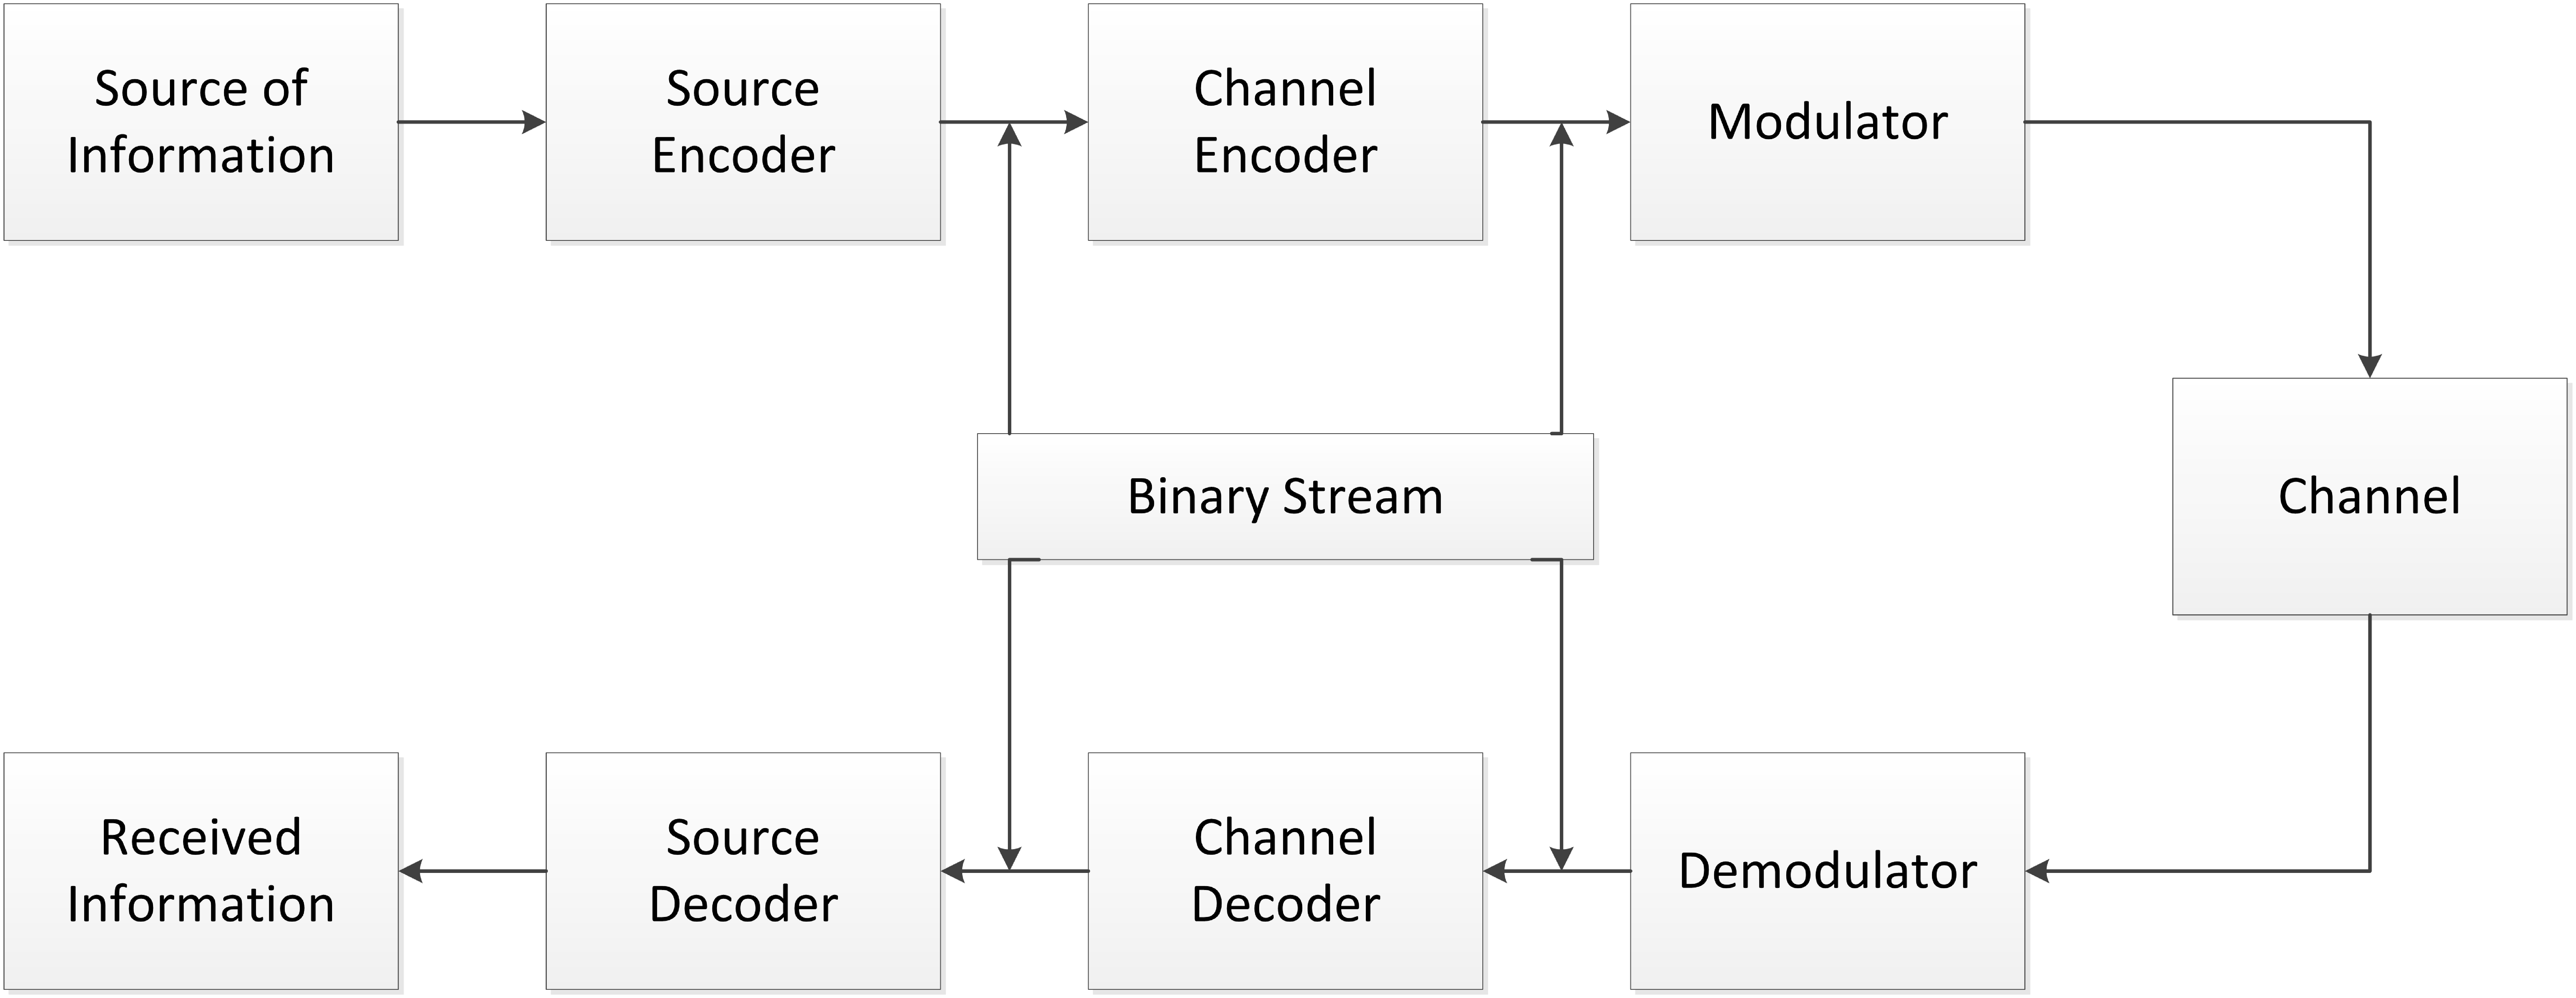
\includegraphics[width=0.85\textwidth]{./figures/digicom_bd}
    \caption{ Digital Communication System Block Diagram
    \label{fig:digcombd}}
\end{figure}

\subsubsection{Source of information}

The sources of information can be of two main kinds, \emph{Analog Information
sources} and \emph{Digital Information Sources}. The Analog information sources
are, for example, microphones and cathodic ray tube televisions, usually any
device that have to reproduce or record anything in the real-world is analogic,
because the real world is analogic. \\

In the other side there are the digital information sources which are composed
by a discrete sequence of symbols, thus the main digital information source is
the PC.

\subsubsection{Source Encoder / Decoder}

The \emph{Source encoder}  and \emph{Source coder} converts the input symbol
sequence into a binary sequence (0 and 1) by assigning code words to the symbols
in the input sequence.\\

If a source set is having hundred symbols, then the number of bits used to
represent each symbol will be 7 because $27=128$ unique combinations are
available. The important parameters of a source encoder are block size, code
word lengths, average data rate and the efficiency of the coder, which is the
actual output data rate compared to the minimum achievable rate.\\

At the receiver, the source decoder converts the binary output of the channel
decoder into a symbol sequence. The decoder for a system using fixed length code
words is quite simple, but the decoder for a system using variable length code
words will be very complex.\\

Aim of the source coding is to remove the redundancy in the transmitting
information, so that bandwidth required for transmission is minimized. Based on
the probability of the symbol codeword is assigned. Higher the probability,
shorter is the codeword.

\subsubsection{Channel Encoder / Decoder}

Error control is accomplished by the channel coding operation that consists of
systematically adding extra bits to the output of the source coder. These extra
bits do not convey any information but helps the receiver to detect and / or
correct some of the errors in the information bearing bits.\\

There are two methods of channel coding:

\begin{enumerate}

  \item \textbf{Block Coding:} The encoder takes a block of ‘k’ information bits
  from the source encoder and adds ‘r’ error control bits, where ‘r’ is dependent
  on ‘k’ and error control capabilities desired.

  \item \textbf{Convolution Coding:} The information bearing message stream is
  encoded in a continuous fashion by continuously interleaving information bits
  and error control bits.

\end{enumerate}


The Channel decoder recovers the information bearing bits from the coded binary
stream. Error detection and possible correction is also performed by the channel
decoder.

\subsubsection{Modulator}

The Modulator converts the input bit stream into an electrical waveform suitable
for transmission over the communication channel, the carrier wave. Modulator can
be effectively used to minimize the effects of channel noise, to match the
frequency spectrum of transmitted signal with channel characteristics, to
provide the capability to multiplex many signals.

\subsubsection{Demodulator}

The extraction of the message from the information bearing waveform produced by
the modulation is accomplished by the demodulator. The output of the demodulator
is bit stream.

\subsubsection{Channel}

The Channel provides the electrical connection between the source and
destination. The different channels are: Pair of wires, Coaxial cable, Optical
fibre, Radio channel, Satellite channel or combination of any of these.\\

The communication channels have only finite Bandwidth, non-ideal frequency
response, the signal often suffers amplitude and phase distortion as it travels
over the channel. Also, the signal power decreases due to the attenuation of the
channel. The signal is corrupted by unwanted, unpredictable electrical signals
referred to as noise. The important parameters of the channel are Signal to
Noise power Ratio (SNR), usable bandwidth, amplitude and phase response and the
statistical properties of noise.

\subsection{Additional Blocks}
%augmented block diagram
\begin{figure}[htbp]
    \centering
    
\includegraphics[width=0.85\textwidth]{./figures/digicom_plus}
    \caption{ Digital Communication System Block Diagram with additional blocks
    \label{fig:digcomplus}}
\end{figure}

Some additional blocks as shown in the block diagram  at figure \ref{fig:digicomplus}
are used in most of digital communication system:

\begin{itemize}

  \item \textbf{Encryptor:} Encryptor prevents unauthorized users from
understanding the messages and from injecting false messages into the system.

  \item \textbf{Multiplexer:} Multiplexer is used for combining signals from
different sources so that they share a portion of the communication system.

  \item \textbf{Demultiplexer:} DeMultiplexer is used for separating the different
signals so that they reach their respective destinations.

  \item \textbf{Decryptor:} It does the reverse operation of that of the Encryptor.

\end{itemize}

\subsection{Synchronization}

Synchronization involves the estimation of both time and frequency coherent
systems need to synchronize their frequency reference with carrier in both
frequency and phase.

\subsection{Advantages and Disadvantages}

Advantages:

\begin{enumerate}

  \item The effect of distortion, noise and interference is less in a digital
  communication system. This is because the disturbance must be large enough to
  change the pulse from one state to the other.

  \item Regenerative repeaters can be used at fixed distance along the link, to
  identify and regenerate a pulse before it is degraded to an ambiguous state.

  \item Digital circuits are more reliable and cheaper compared to analog
  circuits.

  \item The Hardware implementation is more flexible than analog hardware because
  of the use of microprocessors, VLSI chips etc.

  \item Signal processing functions like encryption, compression can be employed
  to maintain the secrecy of the information.

  \item Error detecting and Error correcting codes improve the system performance
  by reducing the probability of error.

  \item Combining digital signals using TDM is simpler than combining analog
  signals using FDM. The different types of signals such as data, telephone, TV
  can be treated as identical signals in transmission and switching in a digital
  communication system.

  \item We can avoid signal jamming using spread spectrum technique.

\end{enumerate}

Disadvantages:

\begin{enumerate}

  \item \textbf{Large System Bandwidth:} Digital transmission requires a large system
  bandwidth to communicate the same information in a digital format as compared to
  analog format.

  \item \textbf{System Synchronization:} Digital detection requires system synchronization
  whereas the analog signals generally have no such requirement.

\end{enumerate}

%-----------------------------------LTE-----------------------------------------

\section{Long Term Evolution} %OK
\label{let:lte}

\subsection{Overview}

Long Term Evolution (LTE) is a standard for wireless communication for high-speed
mobile devices and data terminals. LTE was first introduced in 3GPP Release 8.
It uses orthogonal frequency division multiplexing (OFDM) as its radio access
technology, together with advanced antenna technologies.\\

In addition to LTE, 3GPP also defined IP-based, flat core network architecture.
This architecture was defined as part of the System Architecture Evolution (SAE)
effort specifying the Evolved Packet Core (EPC) network. The LTE-SAE architecture
and concepts have been designed for efficient support of mass-market usage of any
IP-based service. The architecture is based on an evolution of the existing GSM/WCDMA
core network, with simplified operations and smooth, cost-efficient deployment.\\

Moreover, work has also been done by 3GPP in cooperation with 3GPP2 (the CDMA
standardization body) to optimize interworking between CDMA and LTE-SAE. This means
that both CDMA and GSM operators can use the same standard with minor modifications
and thus making the deployment and roaming costs smaller.\\

LTE can be was thought to reduce cost in deployment in legacy systems, as said
before with CDMA and GSM, it can use the legacy systems and adapt itself to work
with them, creating a smooth transition for the network operators \cite{introlte}.\\

The 3GPP radio access  technology was developed towards:

\begin{itemize}
    \item Reduced cost per bit
    \item Increased service provisioning – more services at a lower cost with
    better user experience
    \item Flexible use of existing and new frequency bands
    \item Simplified architecture and open interfaces
    \item Reasonable terminal power consumption
\end{itemize}

The specification work on LTE was completed in March 2009 as the SAE specifications
were included. Below it is possible to see some of the 3GPP Release 8 LTE Requirements:

\begin{itemize}
    \item Increased peak data rates: 100Mbps downlink and 50Mbps uplink
    \item Reduction of Radio Access Network (RAN) latency to 10ms
    \item Improved spectrum efficiency (two to four times compared with HSPA Release 6)
    \item Cost-effective migration from Release 6 Universal Terrestrial Radio
    Access (UTRA) radio interface and architecture
    \item Improved broadcasting
    \item IP-optimized (focus on services in the packet switched domain)
    \item Scalable bandwidth of 20MHz, 15MHz, 10MHz, 5MHz, 3MHz and 1.4MHz
    \item Support for both paired and unpaired spectrum
    \item Support for interworking with existing 3G systems and non-3GPP specified systems.
\end{itemize}

\subsection{Network Architecture}

In parallel with the LTE radio access, the packet core network was implemented as
flat IP-based multi-access core network. The Evolved Packet Core (EPC) network was
designed to optimize network performance, improve cost-efficiency and facilitate
the uptake of mass-market multimedia services.\\

Existing 3GPP (GSM and WCDMA/HSPA) and 3GPP2 (CDMA2000 1xRTT, EV-DO) systems are
integrated to the EPC network through standardized interfaces providing optimized
mobility with LTE. For 3GPP systems this means a signaling interface between the
existing Serving GPRS Support Node (SGSN) to the Mobility Management Entity (MME)
in the EPC network; for 3GPP2 a control signaling interface between the CDMA RAN
and the MME. This integration support both dual and single radio handover, allowing
a flexible migration to LTE.\\

The Home Subscriber Server (HSS) connects to the Packet Core through an IP-based
interface using Diameter, and not SS7, which was used in previous GSM and WCDMA
networks. Network signaling for policy control and charging is already based on
Diameter. This means that all interfaces in the new architecture are IP-based.\\

LTE-EPC has adopted an effective class-based QoS concept. This provides a
foundation for operators to offer service differentiation, depending on the type
of subscription or application.

%figura da rede
\begin{figure}[htbp]
    \centering
    
\includegraphics[width=0.65\textwidth]{./figures/lte_flatepc}
    \caption{ LTE Flat EPC Network Architecture
    \label{fig:lteflatepc}}
\end{figure}

\subsection{Orthogonal Frequency-division Multiplexing Radio Technology} %+/-ok

LTE uses OFDM for the downlink ( from the base station to the terminal or UE).
OFDM meets the LTE requirement for spectrum flexibility and enables cost-efficient
solutions for very wide carriers with high peak rates. It is a well-established
technology: for example, in standards such as IEEE 802.11a/b/g, 802.16, HIPERLAN-2,
DVB and DAB.\cite{introlte} \cite{umtslte}\\

A representation of an OFDM signal can be seen in figure \ref{fig:ofdmfreq}. In
this figure, a signal with 5 MHz bandwidth is shown, but the principle is of
course the same for the other E-UTRA bandwidths. Data symbols are independently
modulated and transmitted over a high number of closely spaced orthogonal
subcarriers.\\

%ofdm scheme
\begin{figure}[htbp]
    \centering
    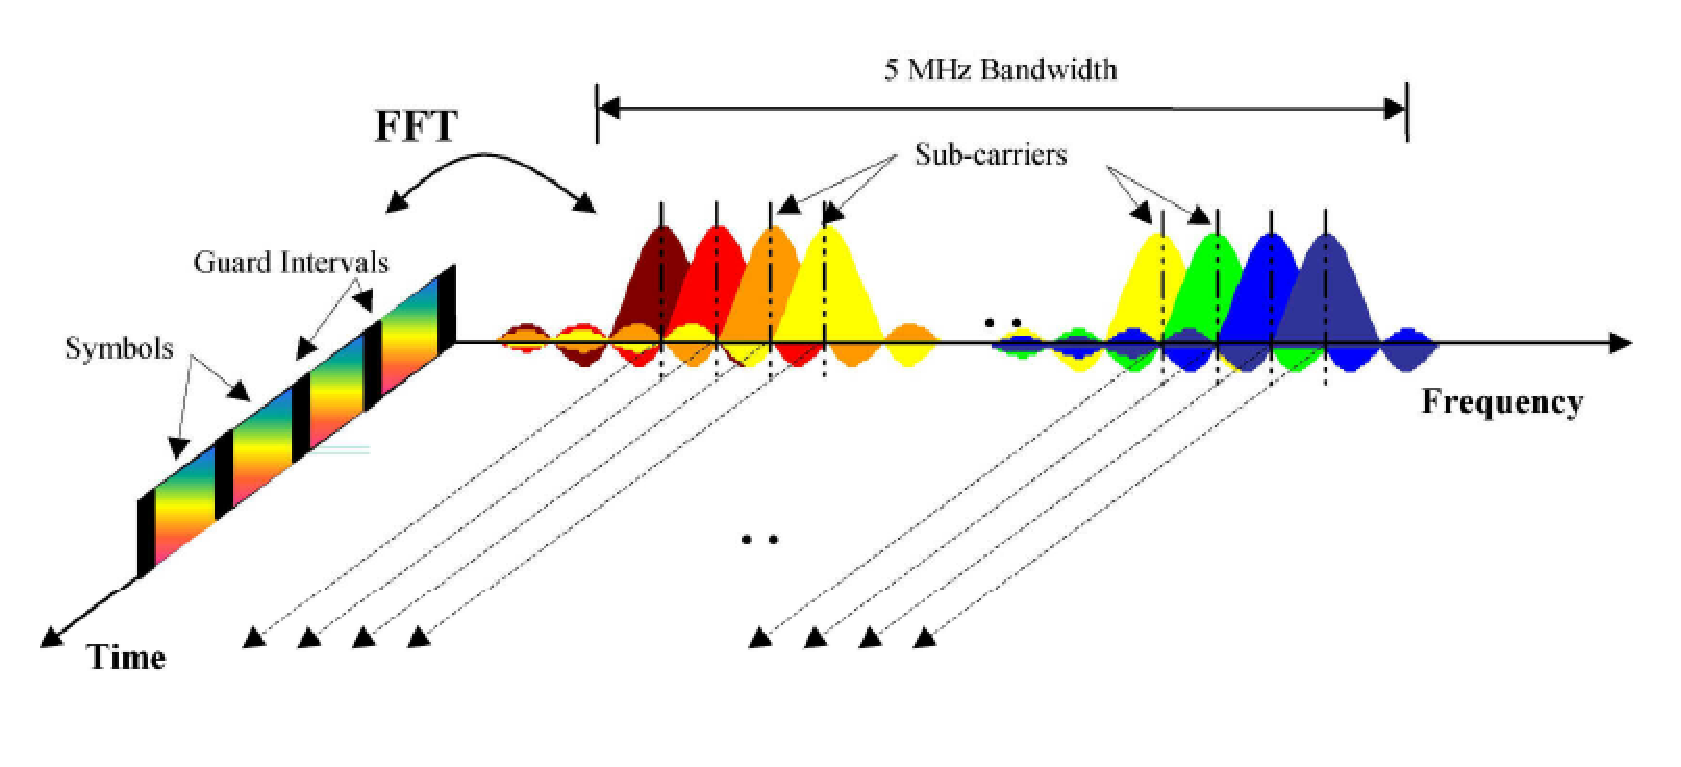
\includegraphics[width=0.65\textwidth]{./figures/ofdm_frequency}
    \caption{ Frequency-Time Representation of OFDM signal
    \label{fig:ofdmfreq}}
\end{figure}

OFDM uses a large number of narrow sub-carriers for multi-carrier transmission.
The basic LTE downlink physical resource can be seen as a time-frequency grid.
In the frequency domain, the spacing between the sub-carriers, $\Delta f$, is 15
kHz. In addition, the OFDM symbol duration time is $\frac{1}{\Delta f} + cyclic prefix$.
The cyclic prefix is used to maintain orthogonality between the sub-carriers even
for a time-dispersive radio channel. One resource element carries QPSK, 16QAM or
64QAM. With 64QAM, each resource element carries six bits.\\

The OFDM symbols are grouped into resource blocks. The resource blocks have a
total size of 180 kHz in the frequency domain and 0.5ms in the time domain. Each
user is allocated a number of so-called resource blocks in the time-frequency grid.
The more resource blocks a user gets, and the higher the modulation used in the
resource elements, the higher the bit rate. Which resource blocks the user gets
at a given point in time, and how many, depends on advanced scheduling mechanisms
in the frequency and time dimensions.\\

Scheduling of resources can be taken every 1ms: that means two resource blocks,
180 kHz wide and in total 1ms in length (called a Scheduling Block). The scheduling
mechanisms in LTE are similar to those used in HSPA, and enable optimal performance
for different services in different radio environments.\\

In the uplink, LTE uses a pre-coded version of OFDM called Single Carrier Frequency
Division Multiple Access (SC-FDMA). This is to compensate for a drawback with normal
OFDM, which has a very high Peak to Average Power Ratio (PAPR). High PAPR requires
expensive and inefficient power amplifiers with high linearity requirements, which
increases the cost of the terminal and drains the battery faster.\\

SC-FDMA solves this problem by grouping together the resource blocks in such a
way that it reduces the need for linearity, and so power consumption, in the
power amplifier. A low PAPR also improves coverage and cell-edge performance.

Since this work shall focus on the Radio Frontend part of the systems, implementing
a downlink scheme, it is interesting to dwell more in the LTE downlink and uplink
schemes.

\subsection{Downlink Scheme}%OK

 The downlink transmission scheme for E-UTRA FDD and TDD modes is based on
conventional OFDM. In an OFDM system, the available spectrum is divided into
multiple carriers, called subcarriers as explained in the previus section. Each
of these subcarriers is independently modulated by a low rate data stream. OFDM
is used as well in WLAN, WiMAX and broadcast technologies like DVB (Digital
Video Broadcasting). OFDM has several benefits including its robustness against
multipath fading and its efficient The user data is carried on the Physical
Downlink Shared Channel (PDSCH). The PDSCH(s) is the only channel that can be
QPSK, 16QAM or 64QAM modulated. The Downlink channel schematic can be seen in
\ref{fig:dlchann}to channels delay spread. The delay spread is the time between
the symbol arriving on the first multi-path signal and the last multi-path
signal component, typically several $\mu s$ dependent on the environment (i.e.
indoor, rural, suburban, city center). The guard interval has to be selected in
that way, that it is greater than the maximum expected delay spread. In E-UTRA,
the guard interval is a cyclic prefix which is inserted prior to each OFDM
symbol.\\

In practice, the OFDM signal can be generated using \textit{IFFT} (Inverse Fast Fourier
Transform) digital signal processing. The \textit{IFFT} converts a number N of complex
data symbols used as frequency domain bins into the time domain signal. Such an
N-point \textit{IFFT} is illustrated in Figure \ref{fig:ofdmsymbol} where $a(mN+n)$
refers to the nth subcarrier modulated data symbol, during the time period $mT_u <
t \le (m+1)T_u$.

%ofdm symbols
\begin{figure}[htbp]
    \centering
    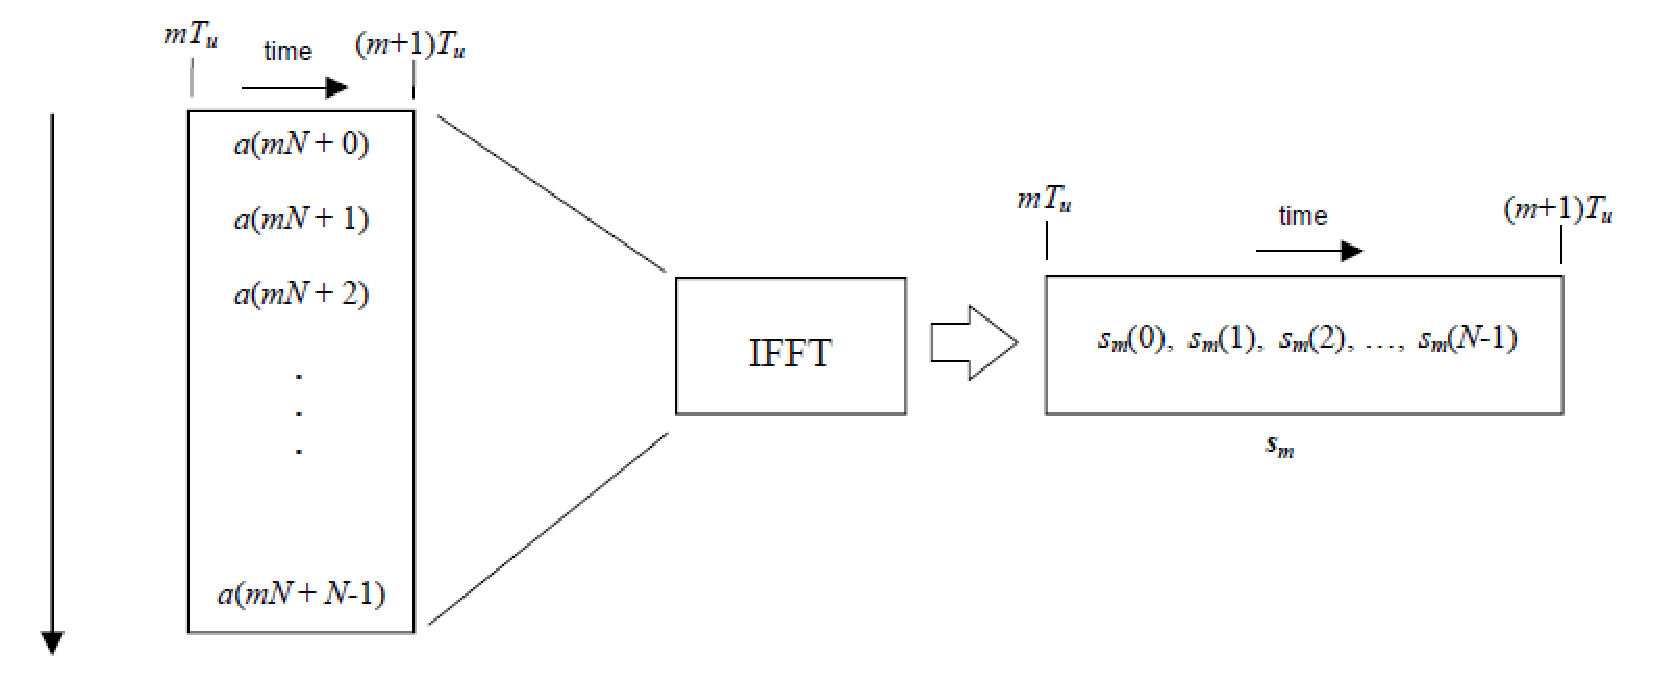
\includegraphics[width=0.65\textwidth]{./figures/ofdm_symbol_gen}
    \caption{ OFDM Symbol Generation
    \label{fig:ofdmsymbol}}
\end{figure}

The vector $sm$ is defined as the useful \textit{OFDM} symbol. It is the time
superposition of the $N$ narrowband modulated subcarriers. Therefore, from a
parallel stream of $N$ sources of data, each one independently modulated, a
waveform composed of N orthogonal subcarriers is obtained, with each subcarrier
having the shape of a frequency sinc function. Figure \ref{fig:ofdmchain}
illustrates the mapping from a serial stream of QAM symbols to N parallel
streams, used as frequency domain bins for the \textit{IFFT}. The N-point time domain
blocks obtained from the \textit{IFFT} are then serialized to create a time domain
signal.

%ofdm signal chain
\begin{figure}[htbp]
    \centering
    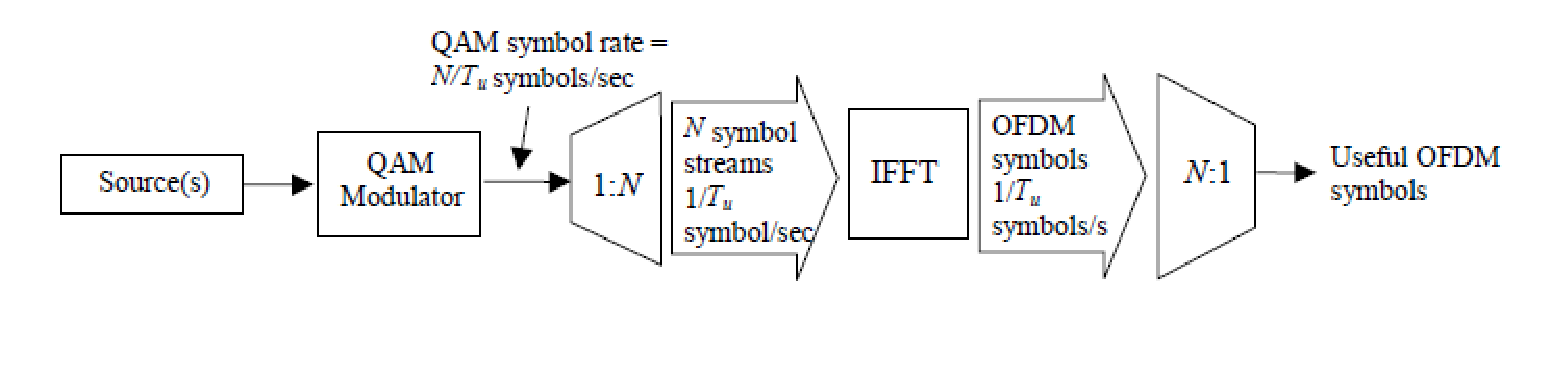
\includegraphics[width=0.65\textwidth]{./figures/ofdm_signal_chain}
    \caption{ OFDM Signal Generation
    \label{fig:ofdmchain}}
\end{figure}

In contrast to an OFDM transmission scheme, \textit{OFDM}A allows the access of multiple
users on the available bandwidth. Each user is assigned a specific time-frequency
resource.

As stated before the data is allocated to a device (User Equipment, UE) in terms
of resource blocks, this means that one UE can be allocated integer multiples of
one resource block in the frequency domain, which representation can be seen in
figure \ref{fig:ofdmresblk}. These resource blocks do not have to be adjacent to
each other. In the time domain, the scheduling decision can be modified every
transmission time interval of 1 ms. All scheduling decisions for downlink and
uplink are done in the base station (enhanced NodeB, eNodeB or eNB). The
scheduling algorithm has to take into account the radio link quality situation
of different users, the overall interference situation, Quality of Service
requirements, service priorities, etc. and is a vendor-specific implementation.\\

%ofdm resource block
\begin{figure}[htbp]
    \centering
    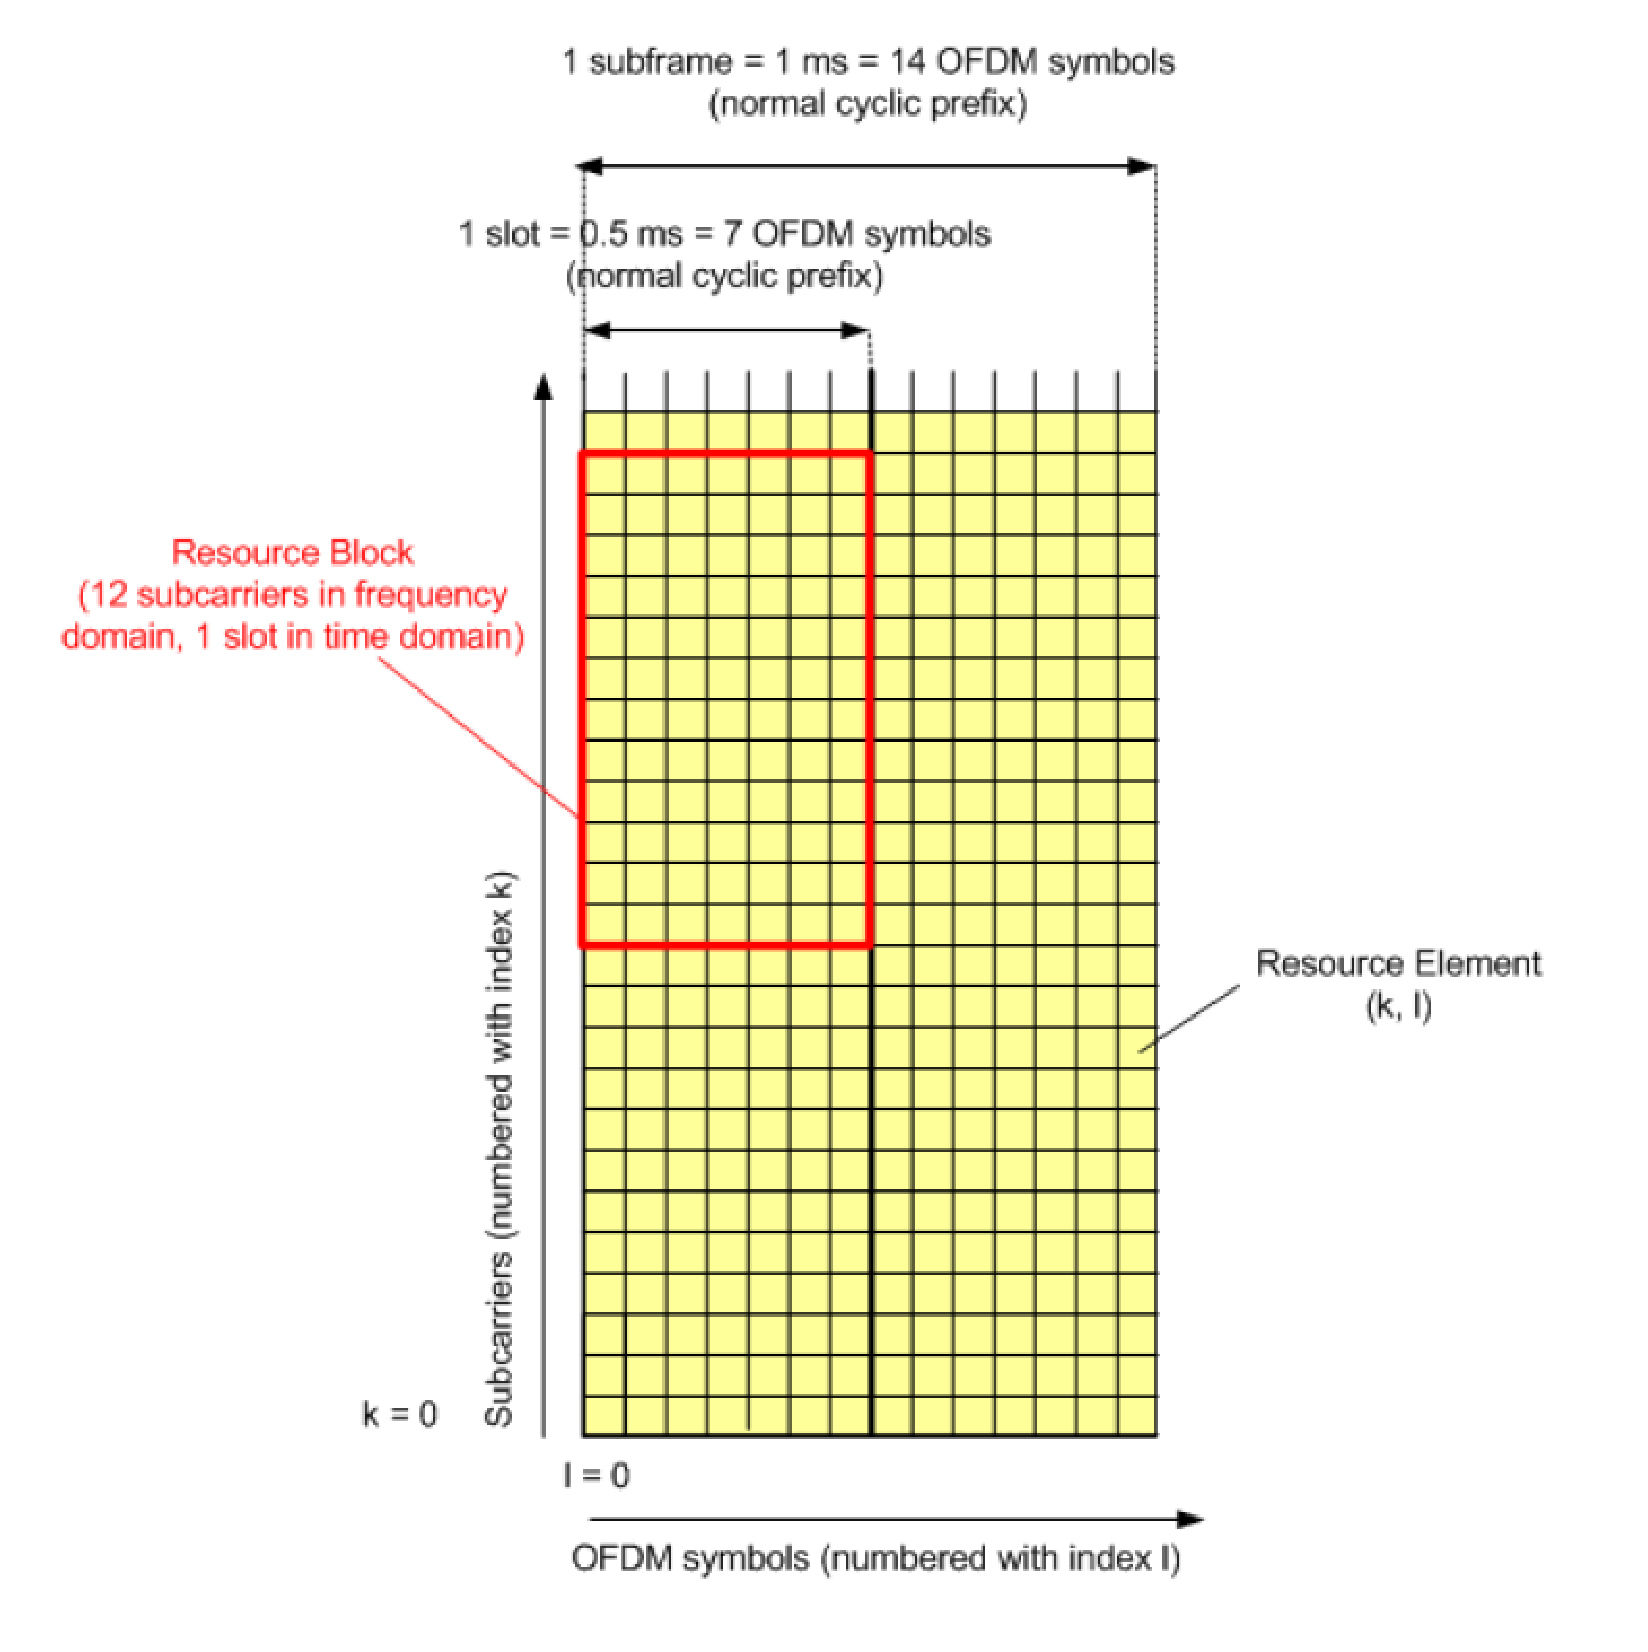
\includegraphics[width=0.65\textwidth]{./figures/ofdm_resource_block}
    \caption{ Resource Block Organization Example
    \label{fig:ofdmresblk}}
\end{figure}

The user data is carried on the Physical Downlink Shared Channel (PDSCH). The
PDSCH(s) is the only channel that can be QPSK, 16QAM or 64QAM modulated. The
Downlink channel schematic can be seen in \ref{fig:dlchann}

%downlink channel figura
\begin{figure}[htbp]
    \centering
    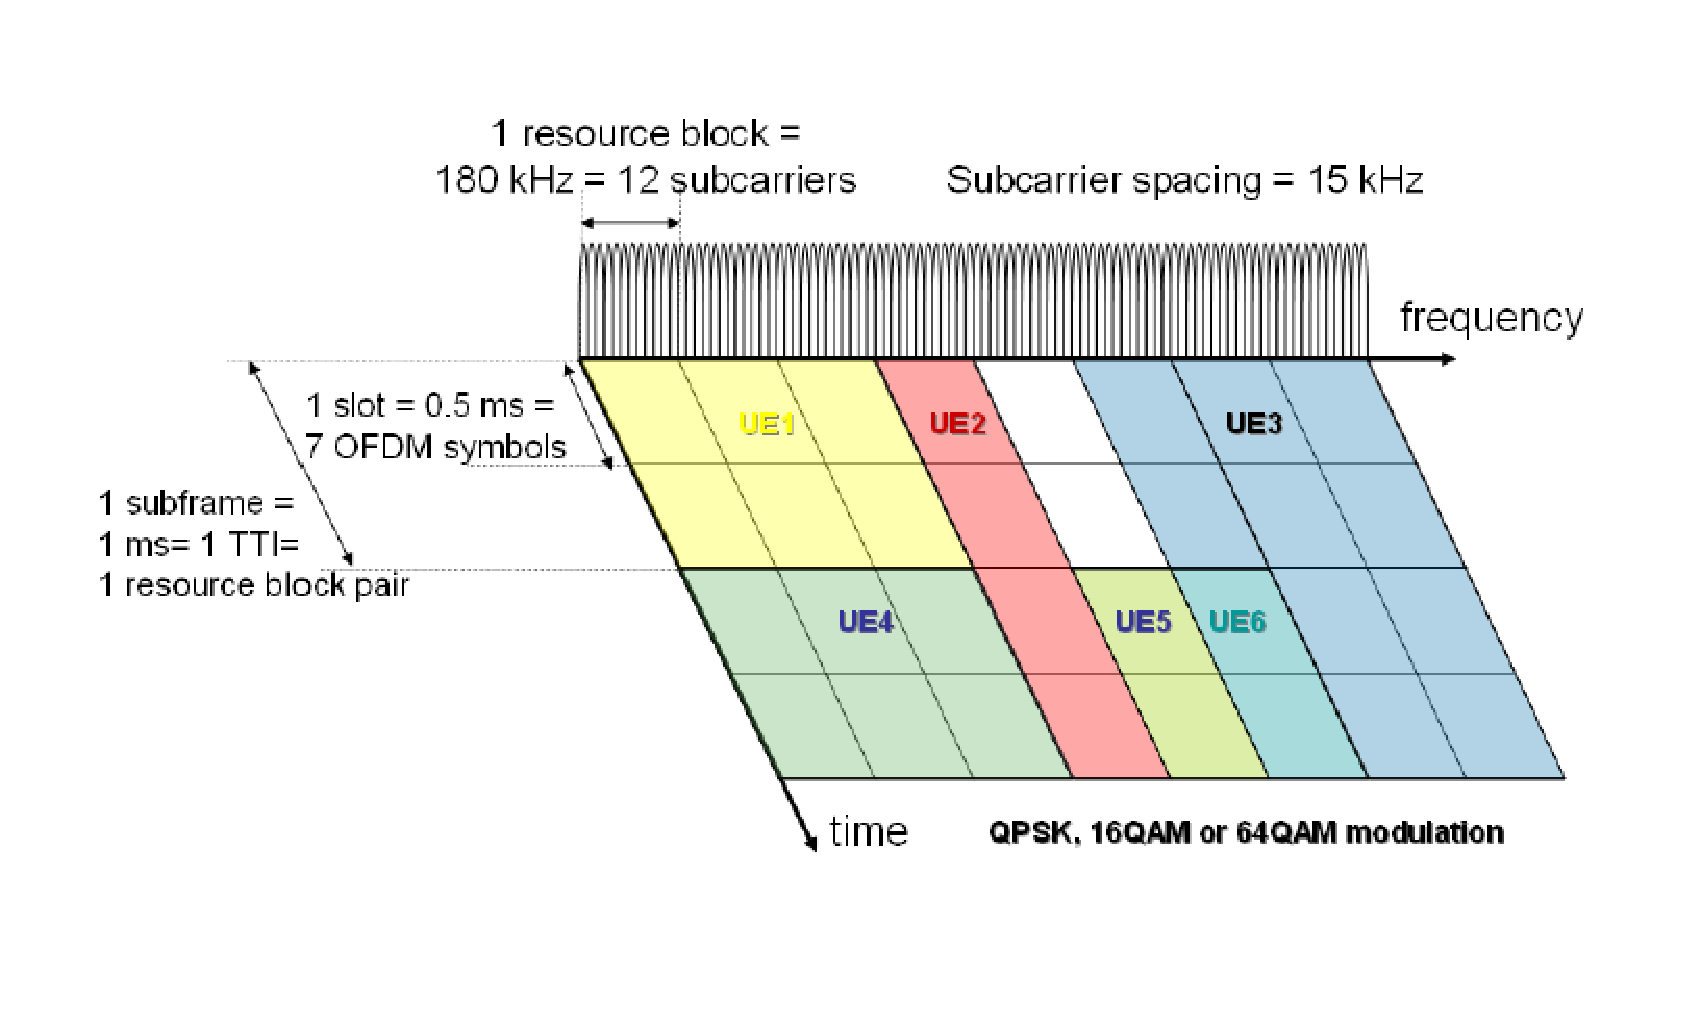
\includegraphics[width=0.65\textwidth]{./figures/downlink_channels}
    \caption{ OFDMA time-frequency multiplexing
    \label{fig:dlchann}}
\end{figure}

\subsection{Uplink Scheme}%ok

 During the study item phase of LTE, alternatives for the optimum uplink
transmission scheme were investigated. While \textit{OFDMA} is seen optimum to fulfill
the LTE requirements in downlink, \textit{OFDMA} properties are less favorable for the
uplink. This is mainly due to weaker peak-to-average power ratio (PAPR)
properties of an \textit{OFDMA} signal, resulting in worse uplink coverage and
challenges in power amplifier design for battery operated handset, as it
requires very linear power amplifiers.\\

Thus, the LTE uplink transmission scheme for FDD and TDD mode is based on SC-
FDMA (Single Carrier Frequency Division Multiple Access) with cyclic prefix.
SCFDMA signals have better PAPR properties compared to an \textit{OFDMA} signal. This was
one of the main reasons for selecting SC-FDMA as LTE uplink access scheme. The
PAPR characteristics are important for cost-effective design of UE power
amplifiers. Still, SC-FDMA signal processing has some similarities with \textit{OFDMA}
signal processing, so parameterization of downlink and uplink can be
harmonized.\\

There are different possibilities how to generate an SC-FDMA signal. DFT-spread-
\textit{OFDM} \textit{(DFT-s-OFDM)} has been selected for E-UTRA. For DFT-s-OFDM, a size-M DFT is
first applied to a block of M modulation symbols. QPSK, 16QAM and 64QAM are used
as uplink E-UTRA modulation schemes, the latter being optional for the UE. The
DFT transforms the modulation symbols into the frequency domain. The result is
mapped onto the available number of subcarriers. For LTE Release 8 uplink, only
localized transmission on consecutive subcarriers is allowed. An N-point \textit{IFFT}
where $N>M$ is then performed as in OFDM, followed by addition of the cyclic
prefix and parallel to serial conversion.

%figura uplink
\begin{figure}[htbp]
    \centering
    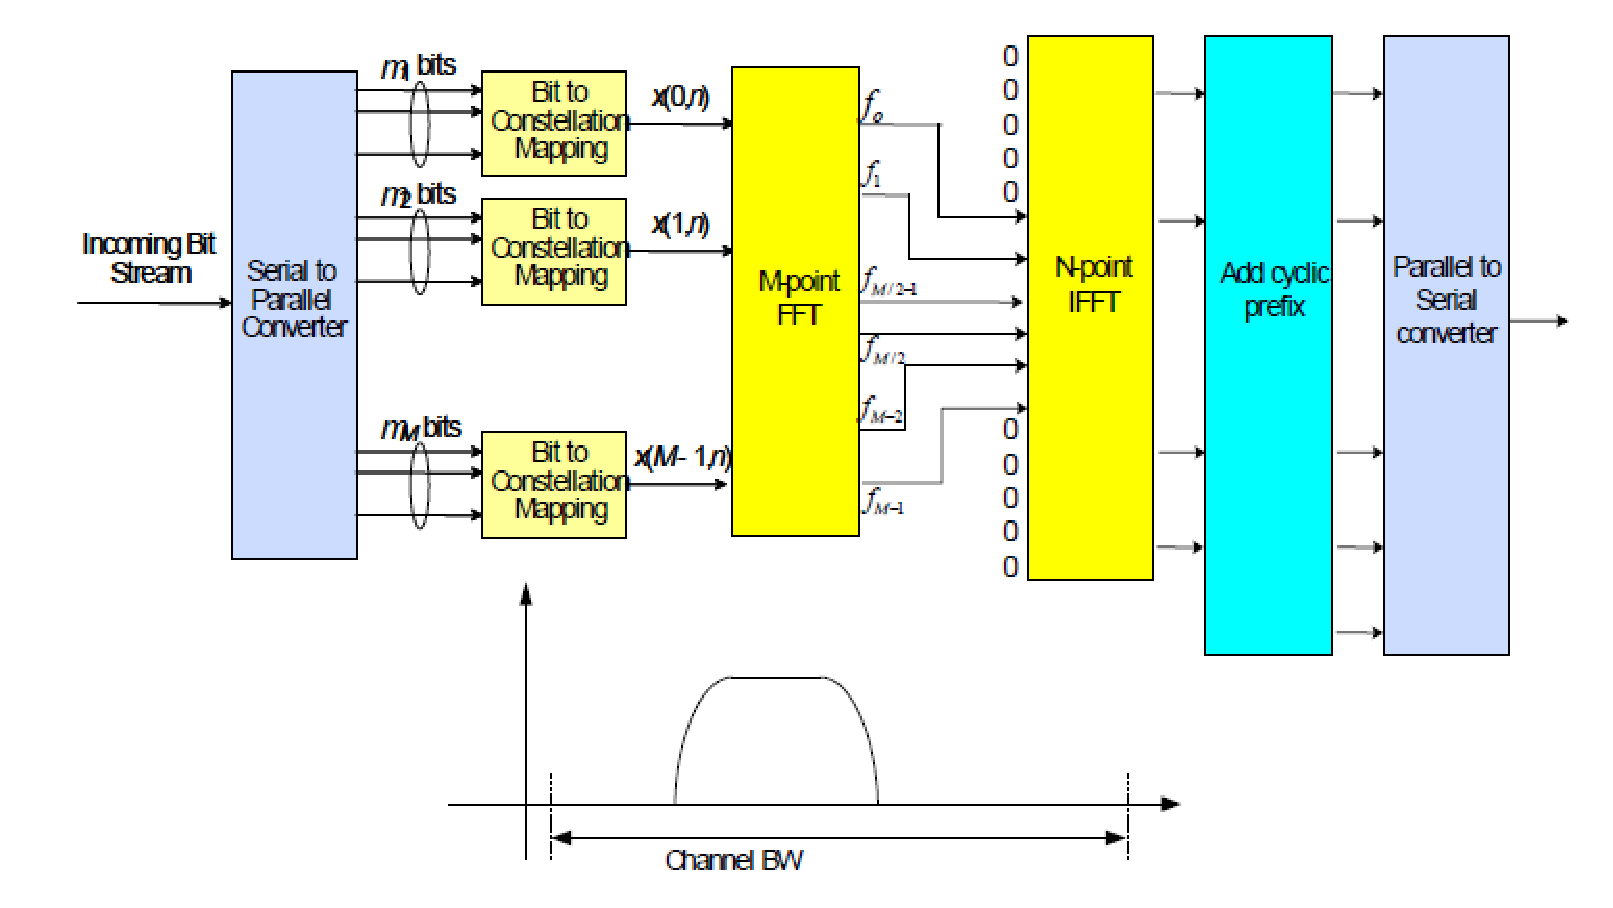
\includegraphics[width=0.65\textwidth]{./figures/uplink_scheme}
    \caption{ LTE Uplink Block diagram of DFT-s-OFDM
    \label{fig:uplinkbd}}
\end{figure}
